%%%% for a4 paper begin
\documentclass[mingoth,oneside]{jsbook}
%%%% for a4 paper end

%%%% for a5 paper begin
%\documentclass[a5paper,mingoth,oneside,14pt]{jsbook}
%\special{papersize=148mm,210mm}
%%%% for a5 paper end

        \usepackage[utf8]{inputenc}
	\usepackage{url}
	\usepackage{titlesec}
	\usepackage[usenames]{color}
	\usepackage{listings,jlisting}
%	\usepackage{listings}
	\usepackage{ascmac}
	\usepackage{fancybox}
	\usepackage{moreverb}
	\usepackage[dvipdfm]{graphicx}
	\usepackage[abs]{overpic}
        \usepackage{ccicons}
	%\usepackage{emathPbb}


\usepackage{soul}
\sethlcolor{GreenYellow}



\newcommand{\colorrule}[1]{%
\begingroup\color{#1}\hrule\endgroup%
}%

\renewcommand{\thesection}{\arabic{section}}
%\renewcommand{\thesubsection}{\arabic{subsection}}

%%%% for a4 paper begin
\setlength{\textwidth}{\fullwidth}
\setlength{\evensidemargin}{\oddsidemargin}
%%%% for a4 paper end

%%%% for a5 paper begin
%\setlength{\fullwidth}{90mm}
%\setlength{\textwidth}{90mm}
%\setlength{\evensidemargin}{-10mm}
%\setlength{\oddsidemargin}{-10mm}
%%%% for a5 paper end


\def\BIG{\fontsize{48pt}{48pt}\selectfont}
\titleformat{\chapter}[frame]
 	{\normalfont}
 	{\filleft\BIG
	\enspace\bfseries{\LARGE 第}\thechapter{\LARGE 章}\enspace}
	{25pt}
	{\huge\bfseries\filleft\vspace{-2mm}}
\titleformat{\section}[hang]
	{\large\gtfamily}
	{\hspace{-1em}}
	%{\hspace{10mm}\thesection}
	{10pt}
	%{}
%%	{\rule[-3mm]{3mm}{8mm} \hspace{-4mm} \rule[-3mm]{25em}{1pt} \hspace{-25em} \Large \ }
	{\rule[-3mm]{3mm}{8mm} \hspace{-4mm} \rule[-3mm]{20em}{1pt} \hspace{-20em} \Large \ }
\titleformat{\subsection}[hang]
	{\large\gtfamily}
	{}
	{10pt}
	{\color{Gray}\hspace{2em}\rule[-2mm]{2mm}{6mm} \hspace{-4mm} \rule[-2mm]{22em}{0.3pt} \hspace{-22em}
	%\color{Gray}
	%\hspace{-5pt}\rule[-1mm]{2mm}{6mm}
	\color{black}
	\large \ }

\newenvironment{result}
{
\begin{center}
\begin{minipage}[c]{42em}
\begin{itembox}[l]{\shadowbox{実行結果}}
}
{
\end{itembox}
\end{minipage}
\end{center}
}



\renewcommand{\lstlistingname}{\small \bf Code} 
\lstset{%
	frame=shadowbox,
	backgroundcolor={\color[gray]{.97}},
	stringstyle={\ttfamily \color[rgb]{0,0,1}},
	commentstyle={\color[rgb]{1,0,1}},
%	commentstyle={\itshape \color[gray]{0.6}},
	identifierstyle={\ttfamily},
%	identifierstyle={\bfseries},
	keywordstyle={\ttfamily \color[rgb]{0,0.5,0}},
%	keywordstyle={\bfseries \color[gray]{0.4}},
	basicstyle={\ttfamily},
%	basicstyle={\bfseries},
	breaklines=true,
%%%%	xleftmargin=4zw,
%%%%	xrightmargin=4zw,
	xleftmargin=0zw,
	xrightmargin=0zw,
	framerule=.2pt,
	columns=[l]{fullflexible},
	numbers=none,
%  stepnumber=5,
	numberstyle={\scriptsize},
	numbersep=1em,
	language={Ruby},
	lineskip=-0.5zw,
	morecomment={[s][{\color[cmyk]{1,0,0,0}}]{/**}{*/}},
	showstringspaces=false,
	tabsize = 5,
%	escapechar=\?,
}


\newcommand{\HRule}{\rule{\linewidth}{0.5mm}}

\title{ {\Huge プログラミング言語入門}}
\author{watanabe}


\begin{document}

% \maketitle
\begin{titlepage}
\begin{center}

% Title
\vspace*{5cm}
\HRule \\[0.4cm]
{ \huge \bfseries プログラミング言語入門}\\[0.4cm]

\HRule \\[1.5cm]

\vspace*{8cm}

% Author and supervisor
\begin{minipage}{0.4\textwidth}
\begin{flushright} \large
{\large 2012/5/25} \\

% lastname \textsc{firstname}
watanabe
\end{flushright}
\end{minipage}


\vspace*{3cm}

\end{center}
\end{titlepage}


% Bottom of the page


\tableofcontents


% \setcounter{page}{0}

\chapter*{はじめに\hspace{-3mm}}

著者が働いている職場には優れた技術者はたくさんいます。ただしそれぞれ受けた教育など背景が異なるため、プログラムは書けてもその基礎となっている計算機科学(コンピュータサイエンス)の理解があやふやな人を、著者は多く見てきました。プログラミングに自信があるという人がもう一歩先に進める道を示したいというのがこの文書を書き始めた動機です。

この文書を読むことで次の効果が得られることを期待しています。
\begin{itemize}
\item プログラミング言語とは何かを深く理解することで、プログラミングのレベルが上がる。
\item “この言語が良い!”と言う時に、シンタックス、ライブラリ、プログラミング言語固有の機能など、どのレベルの機能に言及しているのか区別できる。
\item プログラムがどのように実行されるか理解できる。
\item 関数型言語の中心となる概念を理解できる。
\item λ式とクロージャの違いが説明ができる。
\item 計算機科学の良書である通称SICP\footnote{Structure and Interpretaion of Computer Programs 2nd ed.: 訳本 計算機プログラムの構造と解釈 第2版}という本を読む準備ができる。
\item 友達に“関数型言語の処理系を作ったことがある”と言える ;-)
\end{itemize}
どれか一つにでも魅力を感じれば、この文書の読者の対象と言えるでしょう。

プログラミング言語を理解するために、これから$\mu$SchemeRという独自のプログ
ラミング言語を作成していきます。ものごとの本質を理解するにはその内部が
どうなっているのかを理解することが最も大切だと信じているからです。理解
するためには実際に作ることが一番です。作成する言語は小さな関数型言語を
選びました。作成が簡単にも関わらず強力な機能を持っていること、通常の人
にはなじみが少ないパラダイムである関数型のプログラミング言語を理解する
ことにより、プログラミングの知識に幅を持てるようになるという理由からで
す。

内容が難しすぎそうと不安に思いますか。決してそんなことはありません。こ
の文書の知識の源になっている通称SICPという本は、MITの計算機科学での入門
レベルの講義に使われていました。著者も学部時代に研究室に配属されてまず読
まされた本です。そのくらい、計算機科学に携わる人には基本であり、だから
こそみなさんに知っていただきたい内容なのです。

$\mu$SchemeRを実現するためのプログラミング言語にはRubyを選びました。
Rubyは多くの人が親しんでいる手続き型言語であり、機能も強力なため、本質
的なことを簡潔に説明するのに役立ちます。Rubyに精通していなくとも、
Rubyの簡単な機能しか使いませんし、文章でも説明していきますので気負わず
読み進めてみて下さい。

本文書では、なぜそれが必要なのかをできるだけ記載するようにしました。そ
れが本質を理解するための近道だと思うからです。正解だけを示すのは簡単で
すが、それがなぜ正解なのか、どうやって正解に行き着いたのか、問題は何だっ
たのかを読み取るのは容易ではありません。そこで、まずうまく動作しない例
を挙げ、問題を理解し、それを解決する手段を説明していきます。

本文書で出てくるプログラムをコピー$\&$ペーストしていけば、実行できるよう
になっています。動作することを確認するくらいには役立つでしょう。ただし、
本当に理解したいのであれば、なるべく自分でプログラミングしてみてくださ
い。それもプログラムを見て理解した後は、そのプログラムを見ずに。どこが
理解できないでいるかが明確になるかと思います。

また、本文書は末尾に示すとおり、クリエイティブ・コモンズ 表示 - 非営利
- 継承 3.0 非移植 ライセンスの下に公開しています。改変、再配布をライ
センスに従う範囲内で認めていますので、後輩の教育に有効活用していただければ
こんなにうれしいことはありません。人に教えることが自分で学ぶことの一番
の近道であることを著者はこの文書を書きながらつくづく実感しました。

前振りが長くなってしまいました。それでは、はじめましょう。

\chapter{プログラムと評価\hspace{-3mm}}

\section{プログラミング言語とは}

プログラミング言語とはプログラムを書くための言語です。プログラミング言
語の処理系とは、与えられたプログラムを計算するもので、コンパイラと実行
系の組み合わせで計算したり、インタープリタで計算したりします。本書では
プログラムを逐次解釈
し実行していくインタープリタを作って行きます。これは、与えら
れたプログラムの動作を規定するものですので、見方を変えれば、処理系であ
るインタープリタによりプログラミング言語を定義しているとも言えます
\footnote{これをプログラミング言語を操作的意味論(operetional semantics)で定義すると言います。}。

次にプログラムとは何か、という観点で上の文章を言い換えてみます。プログラム
は計算するための手順をしるしたものと言われていますが、本文書ではこれと
は異なる方法で定義します。すなわち、プログラムが与えられたをとき、
それをどう実行するかを定義します。
今回は、自然言語で書かれた仕様書ではなく、Rubyのプログラムによって、何をプログ
ラムとして受け入れ、それがどう実行されるのかを定めます。これにより、自
然言語に含まれるあいまいさがなく、プログラムとは何かを定めることができます。

はじめから全てのプログラムを対象にすると理解が難しいので、簡単なプログ
ラムの例を示しながら、それが動くように少しずつ機能を追加していきます。

\section{はじめてのプログラムの評価}

最初のプログラムとして次のプログラムを考えます。

\begin{lstlisting}
[:+, 1, 2]
\end{lstlisting}

今までのプログラムと全く異なる記述方法に戸惑うことでしょう。当然です。これは著者が勝手に考えた$\mu$SchemeR(名前も勝手に考えました)というプログラミング言語だからです。気にくわない書き方だと思いますが、この文書を読み終わるころには、自分の好きな書き方へ直す力が身についていると思いますので少しお付き合い下さい。

ただ少し想像力を働かせれば、1と2を足し合わせるプログラムなのだと想像できるのではないでしょうか。そのとおり、正解です。では、“このプログラムを与えられた時にこの結果を求める処理を考えて下さい”と言われたとき、どう答えるでしょうか。“1と2を足し合わせた結果を求める”もしくは“{\tt :+}が先頭にあった時、続く2つの引数の値を足し合わせる”とも言えるでしょう。

では、次のプログラムの結果を求める処理はどうでしょう。

\begin{lstlisting}
[:+, [:+, 1, 2], 3]
\end{lstlisting}

“まず{\tt [:+, 1, 2]}を計算してその結果と3とを足し合わせる”と言えるでしょう。ここで前回の説明に“計算して”という言葉が加わったことに気づいたでしょうか。すなわち、上2つのプログラムの計算結果を求める処理を考えたとき、その処理は{\tt :+}に続く引数を“計算”した後に足し合わせる必要があるのです。通常、我々はこの計算のことを“評価(evaluation)”と言います。したがって、“{\tt :+}が先頭にあった時、続く2つの引数を評価して、その値を足し合わせる”が求める処理です。

% \begin{boxnote}
% {\bf コラム: $\mu$SchemeRのシンタックス} \\

\begin{breakitembox}[l]{\bf コラム: $\mu$SchemeRのシンタックス} 
今回作成するプログラミング言語$\mu$SchemeRでは、{\tt [:+, 1, 2]}などのように
最初に関数を、その後引数を記述します。なぜ、このようなスタイルなのでしょう。他言語のように{\tt x + y * z}と書かかれたものを計算するためには{\tt (x + y) * z}なのか{\tt x + (y * z)}なのかを演算子の優先度を考慮して決める必要があります。さらに言えば、後に出てくるif文も{\tt [:if, :true,  1, 0]}などのように必ず{\tt [}の後に{\tt :if}のようなキーワードが出てくるので、この文字列を見れば通常の関数適用なのか、特殊な構文なのかを簡単に解釈できます。一方で、{\tt if (true) then 1 else 2;}や{\tt x = y + 1;}などのように色々な形の構文を許すとそれがどのような構文なのかを解釈するために多くの計算(字句解析/構文解析)が必要になってきます。計算機がこの処理をせずに人間がこの作業をすることで、計算機側は簡単な処理でそれを解釈できるようになっていると言うわけです\footnotemark[2]。
また、要素は“{\tt ,}”で区切りそれらを“{\tt [}”と“{\tt ]}”で囲みリストを表します。この形式は、Rubyで配列としてそのまま扱えるため、計算機側で余計な処理を考えなくて良くなります。また、記号である{\tt +}や変数である{\tt x}や予約語{\tt if}などは、単語のはじめに{\tt :}をつけてそれぞれ{\tt :+}、{\tt :x}、{\tt :if}と記します。この表記法もRubyでそのままシンボル\footnotemark[3]として扱えるために導入しています。
% \end{boxnote}
\end{breakitembox}
\footnotetext[2]{このことは計算機がすべきことを人間が苦労を強いられているという単純な話ではありません。なぜならプログラミング言語の仕様が単純になるため、結果的に言語仕様を学習する労力が削減されるためです。言語習得の容易さとプログラムの書きやすさのバランスが求められるのかもしれません。}
\footnotetext[3]{Rubyでは{\tt :}に文字列を続けることで、それを定数のように扱えるシンボルという機能が存在します。シンボルを使わない場合、{\tt x}を評価するとRuby上の変数として評価されるため、{\tt x}がRubyで定義されていない場合エラーになるため扱いが面倒となります。}

\setcounter{footnote}{3}

それでは、このプログラムの結果を求める処理をRubyで記述してみましょう。

{\tt \_eval}\footnote{{\tt eval}としないで{\tt \_eval}としているのは、Rubyの組み込み関数として{\tt eval}が定義されているためです。気になる人は、Rubyの{\tt module}機能を使って名前空間を分け、{\tt \_eval}を{\tt eval}として定義しなおして下さい。またその際は、p. \pageref{fun:parse}の{\tt parse}で使われる{\tt eval}は{\tt Kernel::eval}に置き換えて下さい。}は、与えられた式{\tt exp}を評価し、その結果を返します。

式がリストであった場合、最初の要素を関数として、残りを引数として、それぞれを評価してその値を求めます。求めた関数に求めた引数の値を適用(apply)してその結果を{\tt \_eval}の結果とします\footnote{Rubyでは、関数の最後に評価した式の値が関数の返り値になります。一般的に関数型言語では{\tt return} {\it {\tt <}値{\tt >}}と書かずに、このような書き方をします。本書では、関数型言語の考え方に近づくようにこの記述を利用していきます。}。一方、リストでない場合、数字であれば即値として扱い数字そのものを返します。例えば{\tt 2}は2を返します。そうでなければ、組み込み関数とみなし、それに関連付けられた(Ruby上での)関数を返します。

\begin{lstlisting}
def _eval(exp)
  if not list?(exp) 
    if immediate_val?(exp)
      exp
    else 
      lookup_primitive_fun(exp)
    end
  else
    fun = _eval(car(exp))
    args = eval_list(cdr(exp))
    apply(fun, args)
  end
end
\end{lstlisting}

% \begin{boxnote}
% {\bf コラム: プログラムコードと値の区別} \\
\begin{breakitembox}[l]{\bf コラム: プログラムコードと値の区別} 
“{\tt 2}は2を返します”という文章で数字のフォントが違っていることに気づきましたか? {\tt 2}は(現在考えている$\mu$SchemeR)プログラムの、2は(Ruby上での)数値の2を表します。こう記載することによって、プログラムとその評価された値とを区別します。図\ref{fig:uschemer_ruby}を確認してください。
% \end{boxnote}
\end{breakitembox}

以降、上のRubyプログラムで呼ばれている関数を説明していきます。

リストかどうかは配列のインスタンスかどうかで判断しています。

\begin{lstlisting}
def list?(exp)
  exp.is_a?(Array)
end
\end{lstlisting}

組み込み関数は、関数名をキーに、関数本体をその値としたハッシュで保有しま
す。関連付けられている関数はRuby上での関数です。組み込み関数の評価は、
関数名に関連付けられた関数を値として返します。

\begin{lstlisting}
def lookup_primitive_fun(exp)
  $primitive_fun_env[exp]
end

$primitive_fun_env = {
  :+ => [:prim, lambda{|x, y| x + y}],
  :- => [:prim, lambda{|x, y| x - y}],
  :* => [:prim, lambda{|x, y| x * y}], 
}
\end{lstlisting}

{\tt car}はリストの先頭の要素を、{\tt cdr}は先頭の要素以降のリストを取得する関数です。この名前は奇妙\footnote{carはContents of the Address part of Register、cdrはContents of the Decrement part of Register、後で出てくるconsはCONStructから来ています。これらはLispが開発されたIBMの計算機の機械語に由来しています。} ですが、Schemeで使われている名前ですので我慢してください。そのうち慣れてくるでしょう。

\begin{lstlisting}
def car(list)
  list[0]
end

def cdr(list)
  list[1..-1]
end
\end{lstlisting}

引数を評価する{\tt eval\_list}は、リストの要素それぞれを評価したものをリストにしたものです。

\begin{lstlisting}
def eval_list(exp)
  exp.map{|e| _eval(e)}
end    
\end{lstlisting}

そのままの値を返す即値として数字を定義しています。

\begin{lstlisting}
def immediate_val?(exp)
  num?(exp) 
end

def num?(exp)
  exp.is_a?(Numeric)
end
\end{lstlisting}

関数適用は、引数の評価値(Ruby上の値になります)を(Ruby上の)関数へ適用しています。
{\tt fun\_val.call(*args)}は、{\tt fun\_val}というRuby上の関数を引数{\tt args}で呼び出します。{\tt *}は、可変長引数に対応しており、{\tt args}が{\tt [1, 2]}の場合{\tt fun\_val.call(1, 2)}と展開され、{\tt args}が{\tt [1, 2, 3]}の場合{\tt fun\_val.call(1, 2, 3)}と展開されます。

\begin{lstlisting}
def apply(fun, args)
  apply_primitive_fun(fun, args)
end

def apply_primitive_fun(fun, args)
  fun_val = fun[1]
  fun_val.call(*args)
end

def primitive_fun?(exp)
  exp[0] == :prim
end
\end{lstlisting}

実際に、{\tt [:+, 1, 2]}を評価するときの動きを図\ref{fig:uschemer_ruby}を見ながら追ってみましょう。与えるプログラムはリストですので、まず先頭の要素{\tt :+}を評価し、$lambda\{|x, y| x + y\}$を値として得ます。これは、二つの引数を足す(Ruby上の)関数です。次に{\tt 1}, {\tt 2}を評価し、それぞれ(Ruby上での)1, 2を得ます。これを(Ruby上で)適用することで、3を得ます。この値はputsを使って、Ruby上のプログラムで表示することができます\footnote{今回作成している$\mu$SchemeR上でも、表示出来まるようにしますが、後のお楽しみとします。}。

\begin{figure}[htbp]
\begin{center}
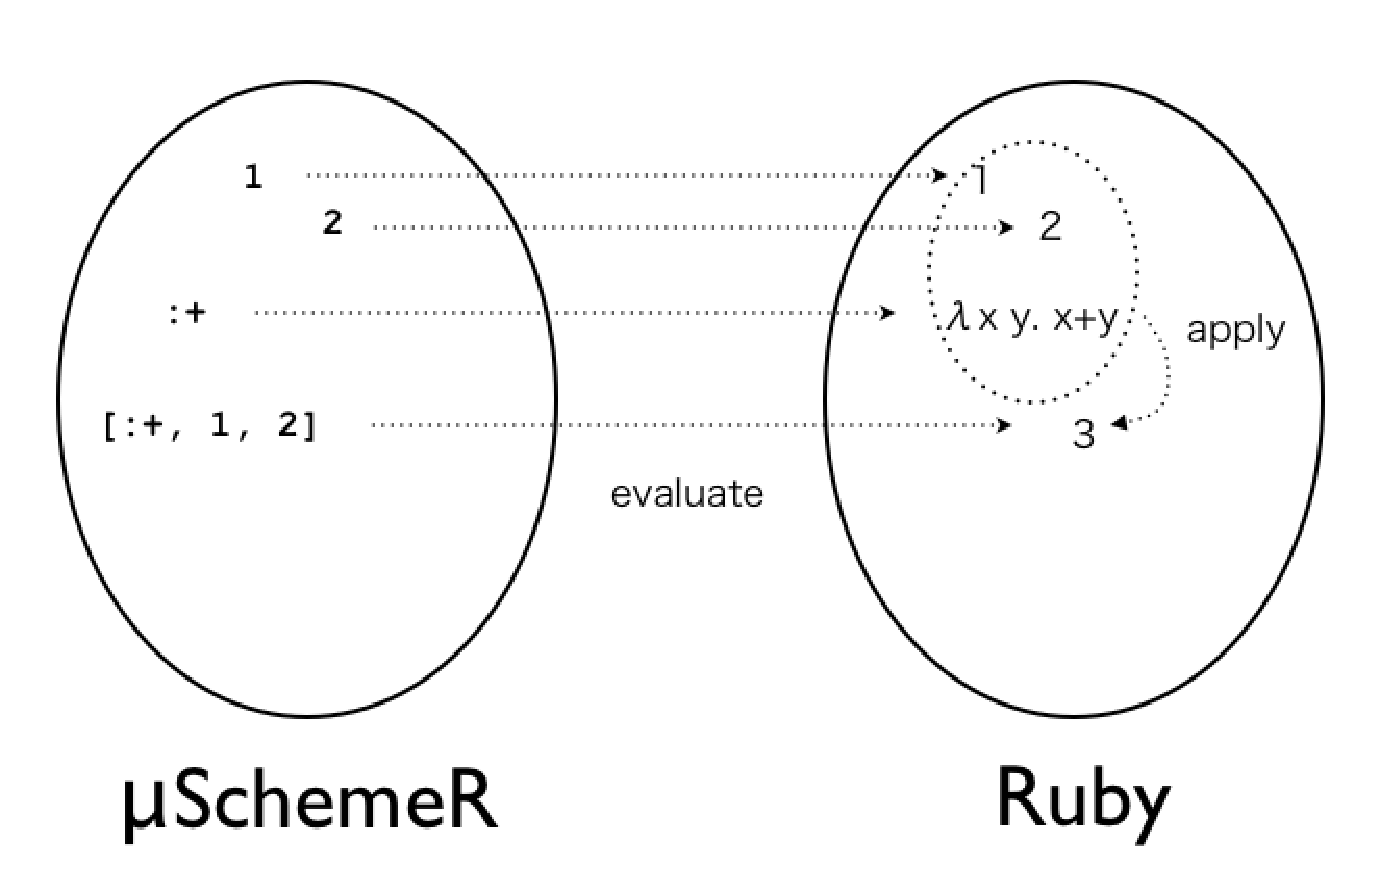
\includegraphics[width=80mm]{images/uschemer_ruby.eps}
\end{center}
\caption{プログラミング言語の世界$\mu$SchemeRと評価値の世界Rubyとの関係}
\label{fig:uschemer_ruby}
\end{figure}


\begin{lstlisting}
puts _eval([:+, 1, 2])
\end{lstlisting}

を実行して3が表示されましたか。おめでとうございます。おそらく、あなたははじめてプログラミング言語のインタープリタを作ったのではないでしょうか。足し算程度しか出来ないプログラミング言語なので実感は無いかもしれませんが、正真正銘のプログラミング言語の処理系です。

{\tt [:+, [:+, 1, 2], 3]}が評価される流れも自分で追ってみて下さい。{\tt \_eval}が再帰的に呼ばれている点が役立っていることに気づけましたか。

\section{まとめ}

この章では次のことを学びました。

\begin{itemize}
\item 簡単なプログラムの計算方法(また、我々はこの計算を“評価”と呼びました)
\item 関数適用の評価方法、すなわち、関数と引数を評価して、得られた関数の評価値に引数の評価値を関数適用するということ
\item プログラムが評価されると(プログラムの実行結果はRubyという)他の世界の値として得られること
\end{itemize}

普段何気なく書いている{\tt x = y;}というプログラムは、実際は右辺をまず評価してその値を左辺の変数のアドレスに格納する、ということを行っています。漠然とは理解していたと思いますが、実際は本章で学んだ評価という考え方などに基づいてプログラムは実行されています。その内部を少し垣間見ることが出来たのではないでしょうか。

\chapter{関数適用の評価\hspace{-3mm}}

この章では関数型言語で大きな位置を占める関数適用の評価方法を学びます。関数適用とは関数に引数を渡して評価することを言います。前章では組み込み関数である{\tt :+}に2つの引数を与え適用した結果として、それらの和を評価値とする関数適用を見てきました。この章では、自分で作った関数についてその適用を考えてみます。

具体的なターゲットは、次のプログラムです。

\begin{lstlisting}
[[:lambda, [:x, :y], [:+, :x, :y]],
         3, 2]
\end{lstlisting}

これは何でしょうか。次のRubyのプログラムはどうでしょう。
\begin{lstlisting}
def add(x, y)
    x + y
end
add(3, 2)
\end{lstlisting}
いずれも、引数を二つとりその和を値とする関数を用意し、その関数に引数3と2を与えて関数適用しているプログラムです。異なる点は、最初のプログラムの関数は名前を持っていません。言わば、関数の中身そのものです。もう少し詳しく説明すると、{\tt [:lambda, [$<parameters>$], $<body>$]}は仮引数{\tt $<parameters>$}でボディが{\tt $<body>$}の関数です。これを関数として、引数を与えることで、前章で学んだ組み込み関数{\tt :+}と同様に関数適用することができます。

このプログラムを実行するためにはどうすれば良いでしょうか。“引数の3, 2を仮引数の{\tt x}, {\tt y}にそれぞれ代入して、中のプログラムを評価する”と考える人が多いのではないでしょうか。おおよそ正しいのですが、考慮すべきポイントがあります。それを見ていきましょう。


\section{環境}
次のプログラムを考えます。

\begin{lstlisting}
[[:lambda, [:x],
  [:+, 
   [[:lambda, [:x], :x], 2],
   :x]], 
 1]
\end{lstlisting}

この時、上の説明でうまくいくか考えて見ましょう。一番外側の{\tt :lambda}の関数適用から考えていきます。{\tt :x}を1に束縛して、{\tt :+}から始まるカッコの中の式を評価します。最初に関数{\tt :+}を評価して、次に3行目の{\tt :lambda}を評価します。この関数は引数をそのまま返しますので、{\tt :x}を2に束縛して関数適用すると2が返ります。問題は次に評価する4行目の{\tt :x}です。この{\tt :x}は1を返すべきですが、{\tt :x}は先ほど2に束縛しています。その結果、2+2すなわち答えが4となってしまうのです(図 \ref{fig:environment1})。

\begin{figure}[htbp]
\begin{center}
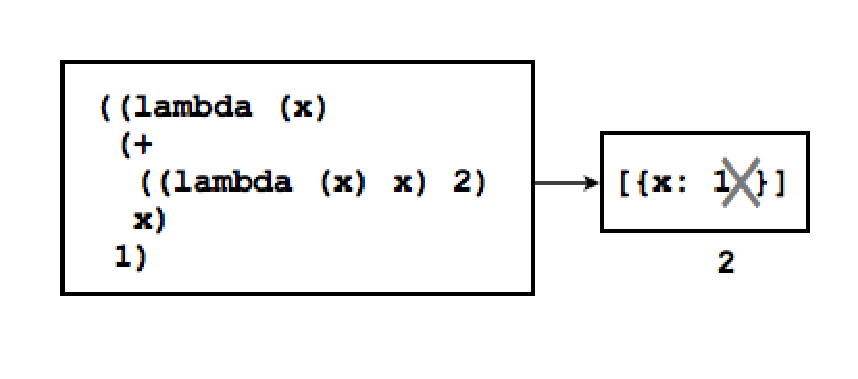
\includegraphics[width=80mm]{images/environment1.eps}
\end{center}
\caption{変数の値を上書きするモデルでの評価のようす。xの値が上書きされるため欲しい値が得られない。}
\label{fig:environment1}
\end{figure}


% \begin{boxnote}
% {\bf コラム: 束縛とは} \\
\begin{breakitembox}[l]{\bf コラム: 束縛とは} 
“{\tt :x}を1に束縛して”という文章が出てきましたが、“束縛”とは何でしょう。変数{\tt :x}と値1とを関連付けるという意味で代入と同じ意味を持ちますが、関数型言語で代入は副作用を引き起こすもの(今は分からないかもしれませんが環境を破壊することとも言います)のことを指すのでそれとは区別して、このように呼びます。また、変数を値に束縛する(bind variable to value)という表現に注意してください。値に対してその名前を一時的につけておいて、後でその名前を通じて値を参照するという使い方をイメージすると良いかもしれません。少し抽象的すぎると思われる人は、Rubyのハッシュを思い出すと良いかもしれません。{\tt h = \{x:1\}}は1という値にxという名前を関連付けておき、後に1を取り出したいときに名前xを使って{\tt h[x]}という形で取り出すことができます。実際、後に出てくるように$\mu$SchemeRでは変数の束縛をハッシュを用いて実装しています。
% \end{boxnote}
\end{breakitembox}

ところで先ほど、“{\tt :x}は1を返すべき”と言いましたが、なぜでしょう。次のプログラムは上のプログラムの内側のλ式の{\tt :x}を{\tt :y}に変えたものです。

\begin{lstlisting}
[[:lambda, [:x],
  [:+, 
   [[:lambda, [:y], :y], 2],
   :x]], 1]
\end{lstlisting}

このプログラムでは明かに求める答えは3です。プログラミング言語にはスコープという考え方があり変数の有効な範囲が決まっています。多くのプログラミング言語では、今回同様、変数の名前を変えただけでプログラムの結果が変わってほしくないので、{\tt :x}は1を返すような言語仕様になっています。今回作成するプログラミング言語もそのような仕様とします。

話を元に戻しましょう。さて、先ほどの答えが4になってしまう問題を解決する
ためにはどうすれば良いのでしょうか。すでにお気づきかもしれませんが、内
側の{\tt :lambda}の{\tt :x}と外側の{\tt :lambda}の{\tt :x}を区別すれば良いのです。内
側の{\tt :lambda}の関数適用を評価しているときは{\tt :x}を2に束縛し、そ
の外側では{\tt :x}を1に束縛するようにします。具体的には、外側
の{\tt :lambda}の関数適用を評価し始めるときに{\tt :x}を1に束縛します。内側の{\tt
:lambda}の関数適用を評価し始めるときに{\tt :x}を2に束縛する環境を新たに用意してそちらを優先し、
その評価が終わればそれを破棄して元の環境に戻すことで、引き続き{\tt :x}を1に束
縛した環境を使うことが出来ます(図 \ref{fig:environment2})。

\begin{figure}[htbp]
\begin{center}
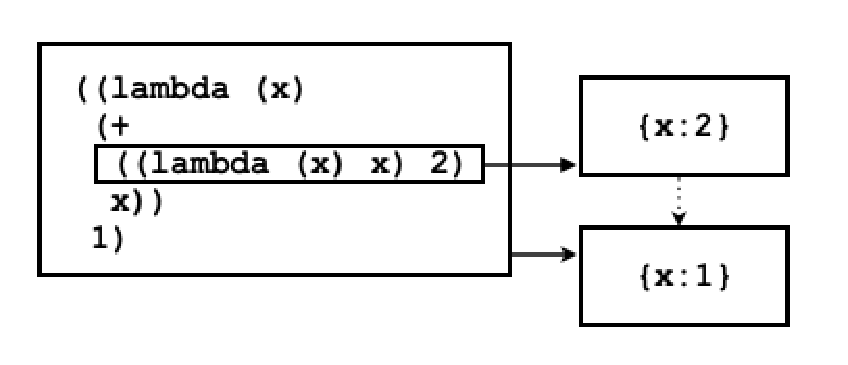
\includegraphics[width=120mm]{images/environment2.eps}
\end{center}
\caption{環境モデル。関数適用時に環境を拡張することで、スコープに応じて、変数が束縛している値を得ることができる。}
\label{fig:environment2}
\end{figure}

ここで新しく環境という言葉を使いました。
環境とは、変数とそれに束縛されている値の組のリストのことです。ここでは、
\{x:1, y:2\}などと表記してxを1にyを2に束縛していることを表し、その組の
リスト[\{x:1, y:2\}, \{x:3\}]で環境を表現することとします。この表現方法
を使えば、最初の{\tt :lambda}を評価しはじめるときは[\{x:1\}]の環境で評価し、
内側の{\tt :lambda}を評価するときは[\{x:2\}, \{x:1\}]という環境で評価します。た
だし同じ変数があった場合、先頭から見ていき最初にマッチした変数に束縛さ
れた値を採用するものとしてします。内側の{\tt :lambda}を評価した後は[\{x:1\}]
という環境に戻すことで、欲しい値が得られることになります。関数呼び出
し時に仮引数と引数の組を環境のスタックに積み、呼び出し終了時にスタック
から取り出すいうイメージです。

以降、環境に関するRubyプログラムを定義していきます。

{\tt lookup\_var}は与えられた環境の中で、指定した変数が束縛している値を見つける関数です。

\begin{lstlisting}
def lookup_var(var, env)
  alist = env.find{|alist| alist.key?(var)}
  if alist == nil
    raise "couldn't find value to variables:'#{var}'"
  end
  alist[var]
end  
\end{lstlisting}

環境の拡張は、与えられた変数をキーに値を格納したハッシュを作り、それを環境の先頭に追加することで実現します。

\begin{lstlisting}
def extend_env(parameters, args, env)
  alist = parameters.zip(args)
  h = Hash.new
  alist.each { |k, v| h[k] = v }
  [h] + env
end
\end{lstlisting}

\section{let式}

少し遠回りになりますが、ここでプログラムを見やすくするためにlet式というものを導入することにします。

\begin{lstlisting}
[:let, [[:x, 3], [:y, 2]],
 [:+, :x, :y]]
\end{lstlisting}

このプログラムは{\tt :x}を3に束縛し、{\tt :y}を2に束縛した環境で、{\tt [:+, :x, :y]}を評価し、その結果をlet式の評価値とする、と解釈します。λ式とどこが違うんだと思うかもしれませんが、そのとおり同じものです。上のlet式は、下の式と同じ意味です。

\begin{lstlisting}
[[:lambda, [:x, :y], [:+, :x, :y]], 3, 2]
\end{lstlisting}

単にプログラムの見やすさから導入した構文ですので、その評価方法も単純です。
{\tt let}は式から仮引数、引数、評価する式を取り出し、λ式に書き換え、評価した値を返します。

\begin{lstlisting}
def eval_let(exp, env)
  parameters, args, body = let_to_parameters_args_body(exp)
  new_exp = [[:lambda, parameters, body]] + args
  _eval(new_exp, env)
end
\end{lstlisting}

{\tt let}から仮引数、引数ならびに評価する本体の式を抜き出します。

\begin{lstlisting}
def let_to_parameters_args_body(exp)
  [exp[1].map{|e| e[0]}, exp[1].map{|e| e[1]}, exp[2]]
end
\end{lstlisting}

let式かを判定する関数も用意しておきます。

\begin{lstlisting}
def let?(exp)
  exp[0] == :let
end
\end{lstlisting}

\section{クロージャ}

それでは覚えたてのlet式を使って次のプログラムを考えてみます。

\begin{lstlisting}
[:let, [[:x, 2]],
 [:let, [[:fun, [:lambda, [], :x]]],
  [:let, [[:x, 1]],
   [:fun]]]]
\end{lstlisting}

このプログラムの結果、どのような答えが返ってきて欲しいですか。まだ{\tt let}に慣れていない人のために読み方を補足すると、{\tt :x}を2に束縛した環境で、{\tt :fun}を{\tt :x}を返す関数に束縛した環境で、{\tt :x}を1に束縛した環境で、{\tt :fun}関数を適用した値を求める、というプログラムです。要は{\tt :x}が{\tt fun:}の呼び出し時の値をとるのか(この場合{\tt :x}は1です)、評価されたときの値をとるのか(この場合{\tt :x}は2です)です。正解は、“プログラミング言語を作る人(すなわち、著者!)が決める"です。そして、その答えは、2です\footnote{このようにプログラムの文脈だけで値を決められるスコープをレキシカルスコープと言い、一方で1が返るようなプログラム実行時の環境を利用する方法をダイナミックスコープと言います。}。

では2を得るためには、どう実現すれば良いでしょう。

λ式を評価するときに、評価時の環境も合わせて持っておくことで、これを実現出来ます。
λ式を評価した時にその結果として、λ式とその時の環境をペア($[(lambda () x), {x:2}]$)で持ち、{\tt fun}はこれを値として束縛します。その後{\tt :x}が1を束縛すると、環境は[\{x:1\}, \{x:2\}]となります。ただし、{\tt fun}を関数適用する際には、先ほどのペアで作成した環境[\{x:2\}]を利用してλ式を評価することで{\tt x}の値は2となります。

まとめると、λ式の評価値はλ式とその評価時の環境のペアです。そのλ式を
関数適用する際には、もう一方のペアである環境で(引数を仮引数に束縛して拡
張して)評価します。このλ式と環境のペアのことをクロージャと呼びます。

実際のRubyのプログラムで実現していきます。

λ式は、λ式と環境でクロージャを作りその評価値とします。

\begin{lstlisting}
def eval_lambda(exp, env)
  make_closure(exp, env)
end

def make_closure(exp, env)
  parameters, body = exp[1], exp[2]
  [:closure, parameters, body, env]
end
\end{lstlisting}

λ式の関数適用は、クロージャからλ式と仮引数および環境を取り出し、取り出した環境を引数と仮引数で拡張して、λ式を評価します。

\begin{lstlisting}
def lambda_apply(closure, args)
  parameters, body, env = closure_to_parameters_body_env(closure)
  new_env = extend_env(parameters, args, env)
  _eval(body, new_env)
end

def closure_to_parameters_body_env(closure)
  [closure[1], closure[2], closure[3]]
end
\end{lstlisting}

最後に、{\tt \_eval}を変更します。式に加えて環境も引数とします。その他、導入したλ式やlet式を扱えるよう変更します。{\tt apply}もλ式の関数適用を扱えるように変更します。

\begin{lstlisting}
def _eval(exp, env)
  if not list?(exp)
    if immediate_val?(exp)
      exp
    else 
      lookup_var(exp, env)
    end
  else
    if special_form?(exp)
      eval_special_form(exp, env)
    else
      fun = _eval(car(exp), env)
      args = eval_list(cdr(exp), env)
      apply(fun, args)
    end
  end
end

def special_form?(exp)
  lambda?(exp) or 
    let?(exp)
end

def lambda?(exp)
  exp[0] == :lambda
end

def eval_special_form(exp, env)
  if lambda?(exp)
    eval_lambda(exp, env)
  elsif let?(exp)
    eval_let(exp, env)
  end
end

def eval_list(exp, env)
  exp.map{|e| _eval(e, env)}
end    

def apply(fun, args)
  if primitive_fun?(fun)
    apply_primitive_fun(fun, args)
  else
    lambda_apply(fun, args)
  end
end
\end{lstlisting}

ユーザプログラムの評価に使う大域環境を用意します。大域環境には組み込み関数を設定します。これにより、組み込み関数を変数と同じように{\tt lookup\_var}で扱うことが出来ます。

\begin{lstlisting}
$global_env = [$primitive_fun_env]
\end{lstlisting}

以降、プログラムを評価して下さいと言われた時は、次のようにプログラムと、
この環境を引数として評価して下さい。

\begin{lstlisting}
exp = [[:lambda, [:x, :y], [:+, :x, :y]], 3, 2]
puts _eval(exp, $global_env)
\end{lstlisting}

クロージャは強力です。次のプログラムを見てください。

\begin{lstlisting}
[:let, [[:x, 3]],
 [:let, [[:fun, [:lambda, [:y], [:+, :x, :y]]]],
   [:+, [:fun, 1], [:fun, 2]]]]
\end{lstlisting}

{\tt :fun}を束縛したλ式中の{\tt :x}はその中で値を束縛していないにも関わらず利用できる点に注意して下さい\footnote{p. \pageref{column:closure}でもう少し強力な例を示します。}。これはクロージャが環境を持っているからです。

\section{評価(eval)と関数適用(apply)}

プログラムの評価方法はこれでほぼ全て学びました。流れをおさらいしてみましょう。プログラムが与えられると、関数ならびに引数の部分に分けられそれぞれを評価します。その後、引数をその関数に適用します。すなわち、仮引数を引数に束縛して、関数のボディを評価します。次は、このボディの中に含まれるプログラムについて、これら一連の処理を繰り返すことになります。このように評価(eval)と関数適用(apply)を再帰的に繰り返しながらプログラムは実行されていくのです。


\section{λ式とクロージャの違い}

ここまで読んできた皆さんなら、λ式とクロージャの違いをよく理解しているでしょう。λ式は単なるプログラムのコードであり、クロージャはλ式とそれを評価した時の環境のペアです。λ式を評価するとクロージャがその評価値となります。このクロージャを関数適用するときは、クロージャ中の環境(仮引数を引数に束縛し拡張した環境)でλ式を評価します。

λ式扱うことができるプログラミング言語は、関数を値として扱う関数、すな
わち高階関数としてFORTRANなど古くから存在してきました。値として扱うとは、
引数や返り値などで使うことが出来ることを言います\footnote{専門用語では、
関数がファーストクラスのオブジェクトであるとも言います。}。高階関数は処理を抽
象化できるため強力な機能となります。例えば、関数の積分値を数値計算で求め
たいとき、求める関数を引数とすることで、各関数毎に同じ処理を書かずにす
みますし、記載した処理がわかりやすくなります。

クロージャは高階関数よりもさらに強力です。ソースコードと環境のペアを値として扱うことで、内部状態を隠蔽することが可能です。最近のプログラミング言語ではクロージャを扱えるものが増えています。ぜひ、その可能性を最大限に利用してプログラミングをより楽しんでください。

\section{まとめ}

この章では次のことを学びました。

\begin{itemize}
\item 関数適用の評価方法
\item クロージャの関数適用は、クロージャ中の環境を仮引数を引数に束縛して拡張した上で、λ式を評価する
\item 環境とは、変数とそれに束縛された値の組のリスト
\item クロージャはλ式と評価時の環境のペア
\item プログラムは評価と関数適用が再帰的に呼ばれながら実行される
\end{itemize}



\chapter{再帰\hspace{-3mm}}

この章では再帰について学びます。ターゲットとなるプログラムは次のものです。

\begin{lstlisting}
[:letrec, 
 [[:fact,
   [:lambda, [:n], [:if, [:<, :n, 1], 1, [:*, :n, [:fact, [:-, :n, 1]]]]]]], 
 [:fact, 3]]
\end{lstlisting}

まずは準備として、$\mu$SchemeRの機能を少し拡張しましょう。

\section{条件式}

次のようなif式で条件を扱えるようにします。

\begin{lstlisting}
[:if, [:>, 3, 2], 1, 0]
\end{lstlisting}

if式の評価はif式から条件、真節、偽節を取得し、条件の評価値が真であれば真節を評価し、偽であれば偽節を評価し、その値を返します。

if式を評価するプログラムを上のとおり書いていきましょう(後で使う{\tt letrec}も合わせて一緒に定義しています)。

\begin{lstlisting}
def special_form?(exp)
  lambda?(exp) or 
     let?(exp) or 
     letrec?(exp) or 
     if?(exp)
end

def eval_special_form(exp, env)
  if lambda?(exp)
    eval_lambda(exp, env)
  elsif let?(exp)
    eval_let(exp, env)
  elsif letrec?(exp)
    eval_letrec(exp, env)
  elsif if?(exp)
    eval_if(exp, env)
  end
end

def eval_if(exp, env)
  cond, true_clause, false_clause = if_to_cond_true_false(exp)
  if _eval(cond, env)
    _eval(true_clause, env)
  else
    _eval(false_clause, env)
  end
end

def if_to_cond_true_false(exp)
  [exp[1], exp[2], exp[3]]
end

def if?(exp)
  exp[0] == :if
end
\end{lstlisting}

if式で分岐するために論理値のリテラルを導入します。
{\tt :true}, {\tt :false}は(Rubyの)true, falseとして解釈するよう大域環境に加えます。

\begin{lstlisting}
$boolean_env = 
    {:true => true, :false => false}
$global_env = [$primitive_fun_env, $boolean_env]
\end{lstlisting}

条件式で扱えるよう、組み込み関数に不等号、等号の演算子を加えます。

\begin{lstlisting}
$primitive_fun_env = {
  :+  => [:prim, lambda{|x, y| x + y}],
  :-  => [:prim, lambda{|x, y| x - y}],
  :*  => [:prim, lambda{|x, y| x * y}],
  :>  => [:prim, lambda{|x, y| x > y}],
  :>= => [:prim, lambda{|x, y| x >= y}],
  :<  => [:prim, lambda{|x, y| x <  y}],
  :<= => [:prim, lambda{|x, y| x <= y}],
  :== => [:prim, lambda{|x, y| x == y}],
}
$global_env = [$primitive_fun_env, $boolean_env]
\end{lstlisting}

\section{再帰}

これで準備が出来ました。いよいよ再帰を見ていきます。次のプログラムを実行してみましょう。

\begin{lstlisting}
[:let, 
 [[:fact,
   [:lambda, [:n], [:if, [:<, :n, 1], 1, [:*, :n, [:fact, [:-, :n, 1]]]]]]], 
 [:fact, 0]]
\end{lstlisting}

1が表示されましたか。では次のプログラムはどうでしょう。

\begin{lstlisting}
[:let, 
 [[:fact,
   [:lambda, [:n], [:if, [:<, :n, 1], 1, [:*, :n, [:fact, [:-, :n, 1]]]]]]], 
 [:fact, 1]]
\end{lstlisting}

エラーになりました。この違いは何でしょう。{\tt :let}を評価すると{\tt :fact}をλ式の値であるクロージャに束縛します。このクロージャの環境には{\tt :fact}は含まれていない点に注意しましょう。{\tt [:fact 1]}として関数適用するとクロージャ中の環境を用いて評価します。評価を進め、if式で偽となると{\tt :fact}を評価しますが、先に述べたようにこの環境には{\tt :fact}は含まれていないためエラーとなるのです(図\ref{fig:let})。すなわち、関数として定義しようとした式の中でその関数の名前を使うにはlet式では不十分であることが分かります。

\begin{figure}[htbp]
\begin{center}
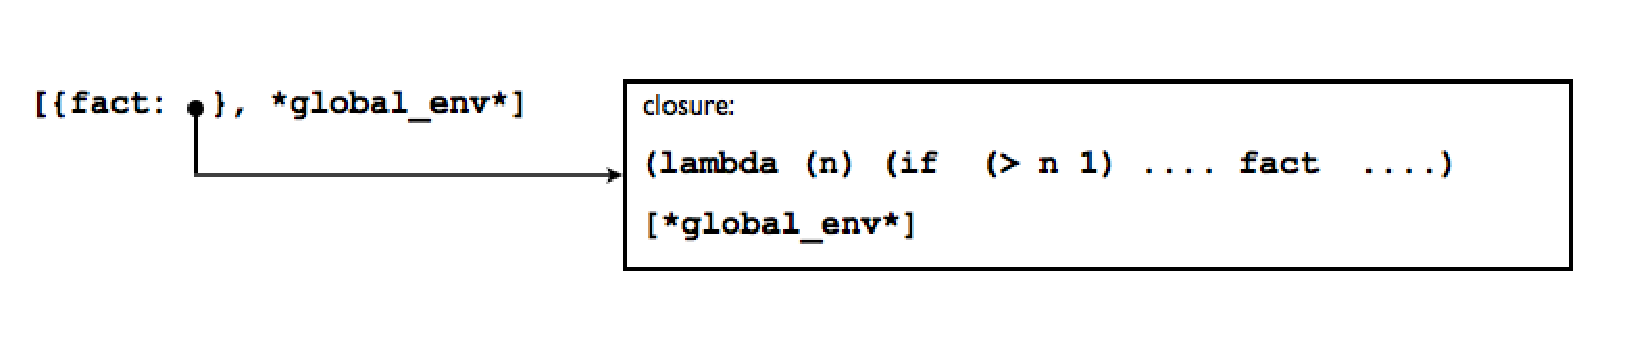
\includegraphics[width=140mm]{images/let.eps}
\end{center}
\caption{{\tt [:fact 1]}評価時の環境のようす。λ式評価時の環境に{\tt fact}がないため、クロージャ内の環境には{\tt fact}は存在せず、{\tt [:fact 1]}でクロージャ中の{\tt fact}を参照しようとするとエラーになる。}
\label{fig:let}
\end{figure}

これを解決するためにはどうすれば良いでしょう。問題は、先に述べたように、{\tt :lambda}を評価してクロージャを作るときに{\tt :fact}が束縛されていないため、返されたクロージャを関数適用に用いると、その中の{\tt :fact}が評価できない点にあります。すなわち、作られるクロージャ中の環境に、それが出来た後で束縛しようとしている{\tt :fact}が含まれている必要があるのです。

これを解決するために、少しトリッキーなことを行います。アイデアは、λ式
を評価しクロージャを作成するときに環境として予め、パラメータ(ここで
は{\tt :fact})の領域を確保しておくことです。ただし、それを束縛する値はまだ定
まっていないので、ダミーの
値を入れておきます(図\ref{fig:letrec}(a))。このとき、パラメータは評価さ
れないためダミーの値でも問題にはなりません。λ式を評価してもλ式の中は
評価されずにクロージャとして返されるためです。λ式の評価値であるクロー
ジャが得られたら、先ほどのパラメータをダミーの値からその値に束縛するよ
うに変更します。(図\ref{fig:letrec}(b))
これでパラメータを評価すると、そのパラメータを環境とし
て含むクロージャを得ることが出来ます。得られた環境を使ってletrec式のボ
ディ{\tt [:fact, 1]}を評価すると(図\ref{fig:letrec}(c))、λ式内の{\tt :fact}
を所望どおり参照することが出来ます。

\begin{figure}[htbp]
\begin{center}
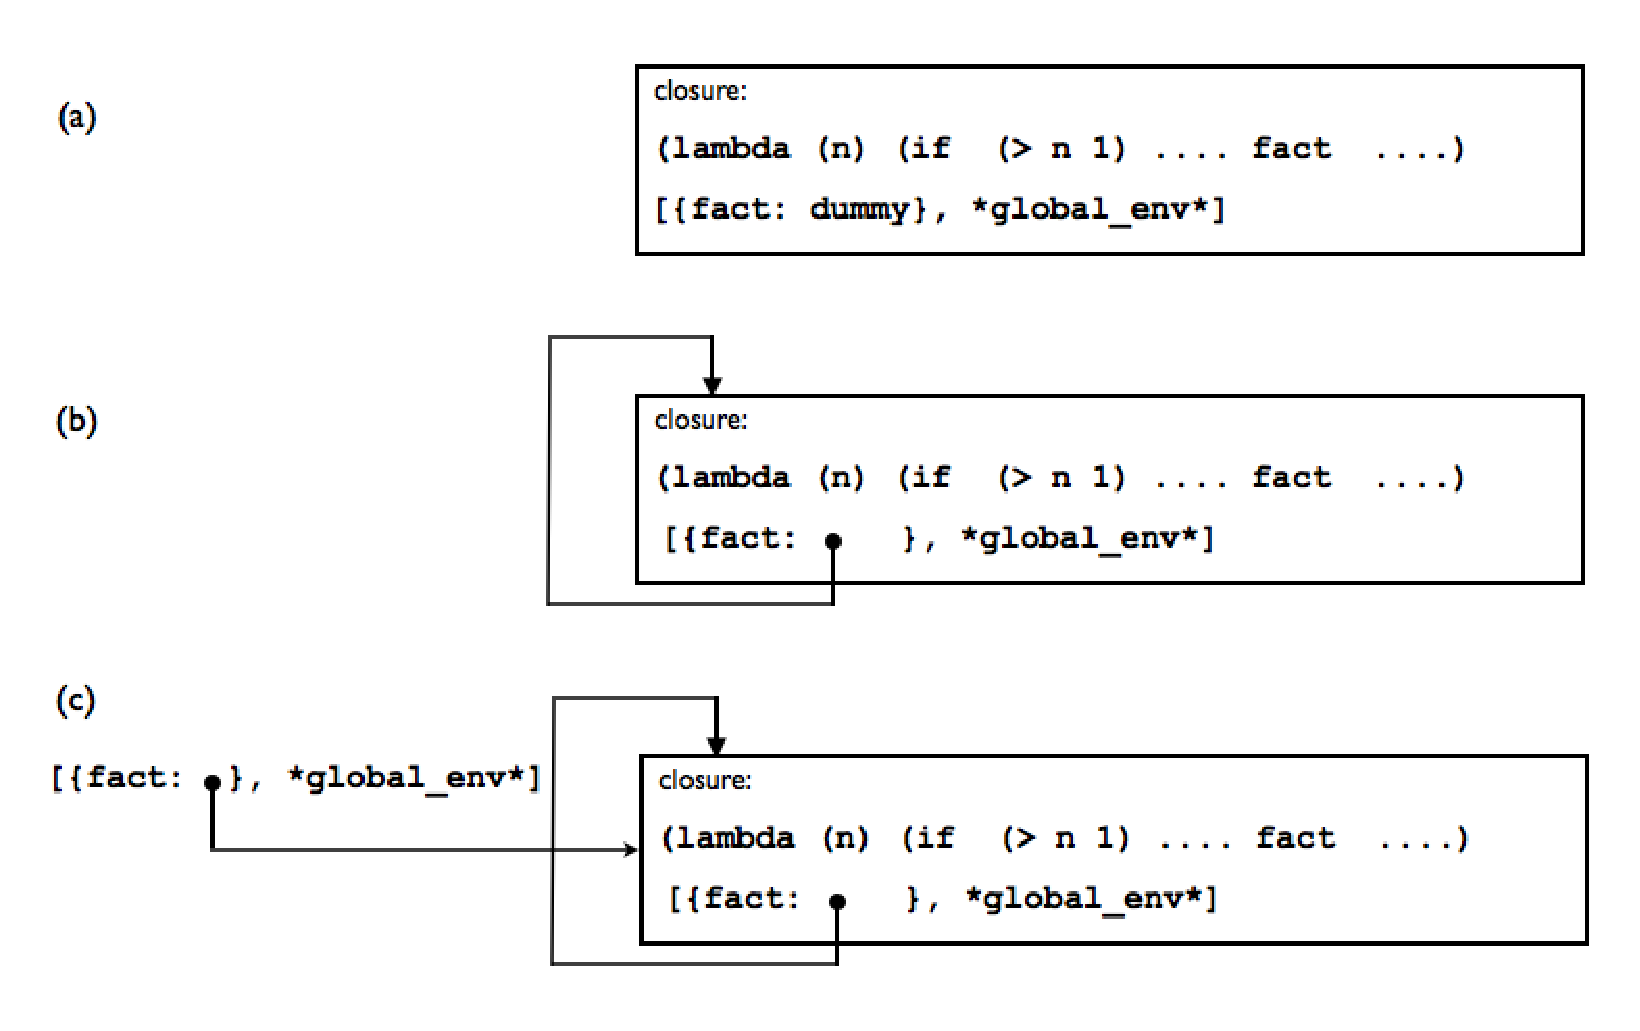
\includegraphics[width=140mm]{images/letrec.eps}
\end{center}
\caption{(a)λ式の評価時の環境に{\tt fact}をダミー値{\tt dummy}に束縛しておき、(b)得られたクロージャの環境の{\tt fact}をクロージャ自身に束縛することで、(c){\tt [:fact 1]}でクロージャの環境内の{\tt fact}が参照可能となる}
\label{fig:letrec}
\end{figure}


以上の機構を実装した再帰を扱う{\tt letrec}を導入します。

\begin{lstlisting}
def eval_letrec(exp, env)
  parameters, args, body = letrec_to_parameters_args_body(exp)
  tmp_env = Hash.new
  parameters.each do |parameter| 
    tmp_env[parameter] = :dummy
  end
  ext_env = extend_env(tmp_env.keys(), tmp_env.values(), env)
  args_val = eval_list(args, ext_env)
  set_extend_env!(parameters, args_val, ext_env)
  new_exp = [[:lambda, parameters, body]] + args
  _eval(new_exp, ext_env)
end

def set_extend_env!(parameters, args_val, ext_env)
  parameters.zip(args_val).each do |parameter, arg_val|
    ext_env[0][parameter] = arg_val
  end
end

def letrec_to_parameters_args_body(exp)
  let_to_parameters_args_body(exp)
end

def letrec?(exp)
  exp[0] == :letrec
end
\end{lstlisting}

それでは、実際に試してみましょう。

\begin{lstlisting}
exp =
  [:letrec, 
   [[:fact,
     [:lambda, [:n], [:if, [:<, :n, 1], 1, [:*, :n, [:fact, [:-, :n, 1]]]]]]], 
   [:fact, 3]]
puts _eval(exp, $global_env)
\end{lstlisting}

正しく、6が表示されましたね。

\section{純粋関数型言語 -- 代入はどこへ?}

おめでとうございます。あなたは、この時点で関数型言語で必要な全ての要素
を学んだと言えます。ただし“最小限の範囲内で”、という限定付きです。今
までに学んできたプログラミング言語は、純粋関数型言語(pure functional
language)と言われ、代入と言った副作用の無い言語です。状態が変わらない、
そもそも状態すら持たないために、変数を、それを束縛している値で入れ替え
ても問題ありません。最適化ではインライン展開と言われる手法です。関数呼
び出しを減らすことが出来るためそれに関わるコストを削減できます。関数呼
び出し時に、環境のスタックを積み上げたことを思い出して下さい。それが不
要になります。もしくは、どの順序で評価してもその値は変わらないため、そ
れぞれを並列に処理することができます。最近、関数型言語が見直されるよう
になってきたのは、このような背景が多分にあります。

そうは言っても手続き型言語で代入を多用している方にとっては、本当に代入
なしで複雑な処理を記述できるのか疑問に思われることでしょう。大丈夫です。
実は、今まで書いてきたRubyのプログラムも簡単に代入なしで書くことが出来
ます。本質的に代入が必要なのは、たった一ヶ所、set\_extend\_env!で使わ
れているハッシュへの代入のみです\footnote{関数名の最後の!は、quoteの
略で、Schemeでは一般的に副作用がある関数の最後にクオート文字!をつけてこ
れを区別しています。この慣習に倣いました。}。他の箇所では引数で渡された配列の中
を代入などにより変更していません。したがってこれ以外の代入は、let式相当の機能
で置き換えても問題ありません(Rubyにはlet式相等の機能がありませんが...)。

本書で考えるプログラミング言語にはあえて代入は導入しません。下手に代入があるとそれに頼ってしまうことがあるからです。新しい関数型言語の考え方に慣れるためにこの言語で色々と処理を書いて見てください。


\section{関数型言語と再帰 -- for文はどこへ?}

再帰は関数型言語にとって大きな意味を持ちます。手続き型言語のfor文など
ループに相当する重要な制御構文です。関数型言語の特徴は、データ構
造に着目して再帰的に処理をすることが多い点です。

実は今回の対象としているプログラミング言語も、数字など基本的な式を組
み合わせて一つのプログラムとなるように設計されています。これ
を式の構成に関する帰納法と呼びます。{\tt eval\_let}などの中で、評価すべ
きプログラムを構成している要素に分け、それぞれの要素に対して再帰的に
{\tt eval}していることを確認してみて下さい。

また、先の例では階乗を求めるプログラムfactを使いました。これも見方を変
えると再帰的に定義された整数に従った構成に関する帰納法とも言えます。整
数
は、0という整数が存在すること、またある整数が存在したとき+1したものが次に大きな整数として
定義されます。この定義に従い、0のときの解を示し、またある整数が与えら
れた時、それより一つ小さい整数の解を用いて求めるものを定義することで、全て
の場合の解を求めることができます。

その他にもまだ扱っていませんが、リストは空リストであるか、リストに先頭
の要素を加えたものである、と再帰的に定義されます。一般的なリスト
を扱う関数はこの定義に従い、与えられたリストが空リストであった場合の処
理と、与えられたリストの最初の要素に対する処理を記載し、残りのリストは
再帰を使って定義します。わかりづらいと思いますので、\ref{chap:extend}章
のp. \pageref{sec:list}のリストの項目(特に{\tt length}関数)を見てからも
う一度この文章を読んで見てください。


\section{まとめ}

この章では次のことを学びました。

\begin{itemize}
\item 再帰関数を実現するための方法
\item 再帰関数の評価値であるクロージャは、その中の環境でクロージャ自身を参照する。
\item これまでに作成してきた$\mu$SchemeRは代入のような副作用がない純粋関数型言語である
\item 手続き言語のループに相当するものを関数型言語では再帰を用いる
\end{itemize}

% % \begin{boxnote}
% {\bf コラム: {\tt letrec}の意味} \\

% 以下、少し高度な話になりますので初めての方は読み飛ばしていただいてかまいません。ここでは{\tt letrec}の意味について少しお話しします。

% 前に、下のプログラムはエラーになることをお話ししました。これは、{\tt :lambda}の中の{\tt :fact}が何も束縛していないためです。
% \begin{lstlisting}
% [:let, 
%  [[:fact,
%    [:lambda, [:n], [:if, [:<, :n, 1], 1, [:*, :n, [:fact, [:-, :n, 1]]]]]]], 
%  [:fact, 1]]
% \end{lstlisting}
% それでは、その{\tt fact}をもう一度同じで{\tt fact}に束縛する、すなわちそのままコードを置き換えると、どうなるでしょう。
% \begin{lstlisting}
%    [[:let, 
%      [[:fact,
%        [:lambda, [:n], 
%         [:if, [:<, :n, 1], 1, 
%          [:*, :n, 
%           [:let, 
%            [[:fact,
%              [:lambda, [:n], [:if, [:<, :n, 1], 1, [:*, :n, [:fact, [:-, :n, 1]]]]]]],
%            [:fact, [:-, :n, 1]]]]]]]], 
%      [:fact, 1]]
% \end{lstlisting}
% 今度は1が表示されたと思います。ただし{\tt [:fact, 2]}を評価すると、今度は一番内側の{\tt :lambda}の中の{\tt fact}が何も束縛していないので、エラーになります。しかし、もう一度今度は一番内側の{\tt :fact}を同じように展開してやると、{\tt [:fact, 2]}まで計算できるようになります。

% このようにn回展開したコードを$\Phi^{n}_{fact}(\emptyset)(x)$とおくと、
% \begin{eqnarray}
%   \Phi^{n}_{fact}(\emptyset)(x)=\left\{ \begin{array}{ll}
%       x! & (0 \leq x < n) \\
%       エラー & (x \geq n) \\
%     \end{array} \right.
% \end{eqnarray}
% となります。

% これを無限回展開したものを、$\Phi^{*}_{fact}$とおくと、これは実質上、factを計算することが出来ます。
% %% $\Phi_{fact}$の話をして、$\Phi^{*}_{fact}(\Phi^{*}_{fact}) = \Phi^{*}_{fact}が成り立つ不動点の話をして、letrecが不動点を求める演算子であるということを言いたい...
% % \end{boxnote}

\chapter{少し言語を拡張して\hspace{-3mm}}\label{chap:extend}
前章までで本質的なことはすべて学んだと言いました。ただし、このままでは
実際のプログラムが書きづらいのも確かです。この章では、我々の言語を書き
やすくするため、いくつかの機能を追加していきます。重要な機能は前章で学
び終わっていますので、気軽に読んでみて下さい。

\section{リスト}\label{sec:list}

ここではリストを扱えるようにします\footnote{今回我々が作成しようとしているSchemeの元言語であるLispという名はList Processingすなわちリスト処理から由来しています。それほど、リストを扱うのが得意な言語なのです。}。ここで紹介する関数は、本来のSchemeではリストに限らず使えるものですが、今回はリストを対象に機能を限定します。

リストは空リストもしくはリストに先頭の要素を加えたものとして構造的帰納法で定義されます。Rubyでは配列で表現します。

{\tt null?}は与えたリストが空リストか調べるものです。空リストは{\tt :nil}で表されます。その他、後で説明するリスト用の組み込み関数も環境として定義しておきます。

\begin{lstlisting}
def null?(list)
  list == []
end

$list_env = {
  :nil   => [],
  :null? => [:prim, lambda{|list| null?(list)}],
  :cons  => [:prim, lambda{|a, b| cons(a, b)}],
  :car   => [:prim, lambda{|list| car(list)}],
  :cdr   => [:prim, lambda{|list| cdr(list)}],
  :list  => [:prim, lambda{|*list| list(*list)}],
}

$global_env = [$list_env, $primitive_fun_env, $boolean_env]
\end{lstlisting}

{\tt cons}は、リストに先頭要素を加えます。リスト以外のものに要素を加えようとすると、我々の不十分な処理系はエラーを返します。

\begin{lstlisting}
def cons(a, b)
  if not list?(b)
    raise "sorry, we haven't implemented yet..."
  else
    [a] + b
  end
end
\end{lstlisting}

(以前定義していますが){\tt car}, {\tt cdr}はそれぞれリストの先頭の要素、および先頭の要素を除いたリストを返します。

\begin{lstlisting}
def car(list)
  list[0]
end

def cdr(list)
  list[1..-1]
end
\end{lstlisting}

{\tt list}は、与えられたリストをそのまま返します。Rubyで可変長引数は配列で渡されますので、配列をリストとして用いているため、そのままの値を使うことができるためです。

\begin{lstlisting}
def list(*list)
  list
end
\end{lstlisting}


\section{定義}

ここでは定義を扱います。次の式を考えてみましょう。
\begin{lstlisting}
[:define, :id, [:lambda, [:x], :x]]
\end{lstlisting}

これは、{\tt :id}を引き数で与えられたものをそのまま返す関数として定義するものです。したがって、その後、下の式を評価すると、
\begin{lstlisting}
[:id, 3]
\end{lstlisting}
3が返されることを期待します。

もう一つ、異なる記述方法の定義を導入します。このプログラムは上の定義と同じ意味を持ちます。
\begin{lstlisting}
[:define, [:id, :x], :x]
\end{lstlisting}

みなさんには、こちらの方がなじみがあるかと思います。関数名に続き仮引数と、それに続く関数のボディから成ります。

これを実装するためにはどうすれば良いでしょうか。変数に定義する値を束縛した環境を付け加えます。ポイントは、その後の評価でもその定義が使えるように環境を書き換える必要があることです。また、すでに変数が束縛されている場合には値を書き換えるようにします。これらは環境を代入により上書きします(関数名が!を使う関数を呼んでいる点に注意しましょう)。

\begin{lstlisting}
def eval_define(exp, env)
  if define_with_parameter?(exp)
    var, val = define_with_parameter_var_val(exp)
  else
    var, val = define_var_val(exp)
  end
  var_ref = lookup_var_ref(var, env)
  if var_ref != nil
    var_ref[var] = _eval(val, env)
  else
    extend_env!([var], [_eval(val, env)], env)
  end
  nil
end

def extend_env!(parameters, args, env)
  alist = parameters.zip(args)
  h = Hash.new
  alist.each { |k, v| h[k] = v }
  env.unshift(h)
end

def define_with_parameter?(exp)
  list?(exp[1])
end

def define_with_parameter_var_val(exp)
  var = car(exp[1])
  parameters, body = cdr(exp[1]), exp[2]
  val = [:lambda, parameters, body]
  [var, val]
end

def define_var_val(exp)
  [exp[1], exp[2]]
end

def lookup_var_ref(var, env)
  env.find{|alist| alist.key?(var)}
end  

def define?(exp)
  exp[0] == :define
end
\end{lstlisting}

準備ができましたので下のようなリストを扱うプログラムをいろいろと実行してみましょう\footnote{実行する前にp.\pageref{sec:quote}で示す{\tt special\_form?}と{\tt 
eval\_special\_form}を追記する必要があります。}。

\begin{lstlisting}
[:define, [:length, :list], 
 [:if, [:null?, :list], 
  0, 
  [:+, [:length, [:cdr, :list]], 1]]]
[:length, [:list, 1, 2]]
\end{lstlisting}

\section{cond式}

条件分岐はif式で記述出来ますが、条件が多くなると、ifのネストが深くなり、プログラムが見づらいものになっていきます。
そこで次のような式を実行できるcondを導入します。

\begin{lstlisting}
[:cond, 
 [[:>, 1, 1], 1],
 [[:>, 2, 1], 2],
 [[:>, 3, 1], 3],
 [:else, -1]]
\end{lstlisting}

この式は上から、リストの左の条件式を順に評価し、真になればその右の式を評価値をcond式の値とします。偽であれば、その下のリストに対して同様のことを行います。{\tt :else}があった場合は、その右の式を値とします。リストはいくつあっても構いません。この場合は2が返り値となります。

この実装はif式に書き換え、それを評価するだけです。

\begin{lstlisting}
def eval_cond(exp, env)
  if_exp = cond_to_if(cdr(exp))
  eval_if(if_exp, env)
end

def cond_to_if(cond_exp)
  if cond_exp == []
    ''
  else
    e = car(cond_exp)
    p, c = e[0], e[1]
    if p == :else
      p = :true
    end
    [:if, p, c, cond_to_if(cdr(cond_exp))]
  end  
end

def cond?(exp)
  exp[0] == :cond
end
\end{lstlisting}

\section{パーサー}

ここまでプログラムを書いてきて、プログラムが書きづらかったことでしょう。プログラムをRubyで評価しやすいように、Rubyの配列を用いてパーサーを省略するとともに、Rubyのシンボルを用いてシンボルテーブルを省略していたためです。LispやSchemeはよくカッコのお化けと言われますが、今まさにその表記法に移る時が来ました。

次のように“{\tt ()}”を使う本来のSchemeの記述方法プログラムを
Rubyの文字列として入力すると、今までと同じように“{\tt []}”や“{\tt ,}”を使った
Rubyのデータ型に変換するものを作ります。変換後のデータを評価させれば
今までどおりの結果が得られますので、ユーザは“{\tt ()}”を使う普通の
Schemeのプログラムを入力できるようになります。

\begin{lstlisting}
_eval(parse('(define (length list) (if  (null?, list) 0 (+ (length (cdr list)) 1)))'), 
      $global_env)
puts _eval(parse('(length (list 1 2 3))'), $global_env)
\end{lstlisting}

これは、“{\tt (}”, “{\tt )}”を “{\tt [}”, “{\tt ]}”
に、変数をRubyのシンボルに置き換えるため“{\tt :}”を変数の先頭に追加し、空白を“{\tt ,}”に置換するより実現します。

\label{fun:parse}

\begin{lstlisting}
def parse(exp)
  program = exp.strip().
    gsub(/[a-zA-Z\+\-\*><=][0-9a-zA-Z\+\-=!*]*/, ':\\0').
    gsub(/\s+/, ', ').
    gsub(/\(/, '[').
    gsub(/\)/, ']')
  eval(program)
end
\end{lstlisting}

\section{quote} \label{sec:quote}

次に追加する機能は{\tt quote}です。次のようにリストを引数として与えるときなどで便利です。

\begin{lstlisting}
puts _eval(parse('(length (quote (1 2 3)))'), $global_env)
\end{lstlisting}

{\tt quote}の引数は評価せずに引数をそのまま評価値として返します\footnote{{\tt quote}は通常、{\tt '}を使って簡易に記載できます。すなわち、{\tt (quote 1 2 3)}は{\tt '(1 2 3)}と同じものです。これは処理系が{\tt '}を読み込んだ時に、{\tt quote}に展開することで実現されています。腕に自信のある方はぜひこの機能の実装にチャレンジしてみて下さい。Ruby 1.9から正規表現でカッコの対応付けが可能になっています。}。

その他の例を挙げてみます。プログラムを引数とする関数を書きたい場合、通常であれば引数が評価されてその関数に渡されます。しかし、その評価の方法をその関数で書きたいので、評価値ではなく式そのものを関数に渡したいのです。このような場合に{\tt quote}は役立ちます。

\begin{lstlisting}
def eval_quote(exp, env)
  car(cdr(exp))
end

def quote?(exp)
  exp[0] == :quote
end
\end{lstlisting}

それでは今まで、拡張してきた機能が動作するようにしましょう。

\begin{lstlisting}
def special_form?(exp)
  lambda?(exp) or 
    let?(exp) or 
    letrec?(exp) or 
    if?(exp) or 
    cond?(exp) or 
    define?(exp) or 
    quote?(exp)
end

def eval_special_form(exp, env)
  if lambda?(exp)
    eval_lambda(exp, env)
  elsif let?(exp)
    eval_let(exp, env)
  elsif letrec?(exp)
    eval_letrec(exp, env)
  elsif if?(exp)
    eval_if(exp, env)
  elsif cond?(exp)
    eval_cond(exp, env)
  elsif define?(exp)
    eval_define(exp, env)
  elsif quote?(exp)
    eval_quote(exp, env)
  end
end
\end{lstlisting}

\section{REPL}

最後にインタープリタと呼ばれるにふさわしい処理を付け加えます。インタープリタはユーザと対話しながらプログラムを作成することができる点に特徴があります。この機能、すなわち、ユーザから入力を読み取り(Read)、その結果を評価し(Eval)、その結果を表示する(Print)ことを繰り返す(Loop)機能です。これは頭文字をとって、REPLとも呼ばれます。

実現は上の機能をそのまま単純に実装します。ここで、{\tt pp}\footnote{{\tt pretty printの略です。}}という式を整形する処理を新たに定義しています。

\begin{lstlisting}
def repl
  prompt = '>>> '
  second_prompt = '> ' 
  while true
    print prompt
    line = gets or return
    while line.count('(') > line.count(')') 
      print second_prompt
      next_line = gets or return
      line += next_line
    end
    redo if line =~ /\A\s*\z/m 
    begin
      val = _eval(parse(line), $global_env)
    rescue Exception => e
      puts e.to_s
      redo
    end
    puts pp(val)
  end
end

def closure?(exp)
  exp[0] == :closure
end

def pp(exp)
  if exp.is_a?(Symbol) or num?(exp)
    exp.to_s
  elsif exp == nil
    'nil'
  elsif exp.is_a?(Array) and closure?(exp)
    parameter, body, env = exp[1], exp[2], exp[3]
    "(closure #{pp(parameter)} #{pp(body)})"
  elsif exp.is_a?(Array) and lambda?(exp)
    parameters, body = exp[1], exp[2]
    "(lambda #{pp(parameters)} #{pp(body)})"
  elsif exp.is_a?(Hash)
    if exp == $primitive_fun_env
      '*prinmitive_fun_env*'
    elsif exp == $boolean_env
      '*boolean_env*'
    elsif exp == $list_env
      '*list_env*'
    else
      '{' + exp.map{|k, v| pp(k) + ':' + pp(v)}.join(', ') + '}'
    end
  elsif exp.is_a?(Array)
    '(' + exp.map{|e| pp(e)}.join(', ') + ')'
  else 
    exp.to_s
  end
end
\end{lstlisting}

それでは実行してみましょう。

\begin{lstlisting}
>> repl
>>> (define (fib n) (if (< n 2) n  (+ (fib (- n 1)) (fib (- n 2)))))
nil
>>> (fib 10)     
55
\end{lstlisting}

実行出来ました。

今までよりはずいぶん楽になるのではないでしょうか。

\section{その他}
他に不便なところはありませんか。まだまだあるでしょう。実現していない機能は多々あります。{\tt named let}や{\tt let*}などの機能を調べその実装にトライしてみて下さい。
友達に速度が遅いと言われたら、コンパイラを作りましょう。Haskellのように遅延評価でないとと言われたら、遅延評価にしてしまいましょう。他の言語のこの機能がない、と言われたら、自分で追加してしまいましょう。自分でプログラミング言語を作ったからこそ味わえるおもしろさです。大いに使い倒して下さい。


\section{まとめ}
この章では、プログラミングを便利にするような次の機能を実現しました。
\begin{itemize}
\item defineによる定義
\item リスト
\item cond式
\item パーサー
\item quote
\item REPL
\end{itemize}



\chapter{次のステップ\hspace{-3mm}}

\section{Scheme in $\mu$SchemeRにチャレンジ}
既にみなさんは関数型言語の本質は理解していますが、まだ関数型言語のプロ
グラミングに慣れているとは言えません。プログラミングは書いて慣れるもの
ですので、プログラミング言語の原理を理解しているだけでは不十分です。様々
なプログラムを書いてみて、その考え方を学んでください。

その教材を一つご紹介します。今回はRubyを用いてSchemeのサブセットを実現
しました。このRubyのプログラムをSchemeで書いて見ましょう。しかも、ただ
Schemeで書くのはつまらないので、今回開発した$\mu$SchemeRで動作させて下
さい。これが実現すれば、Ruby上で$\mu$SchemeRが動き、その上
で今回作成する(今回Rubyで作成したのと同等の)Scheme処理系が動き、その上で
ユーザが与えたSchemeプログラムが解釈、実行されることになります。想像した
だけでエキサイティングになりませんか。

足りない機能があれば、$\mu$SchemeRの処理系をRubyで書き足しながら
実現してみてください。

実現する上でのヒントです。2ヵ所で代入が必要になります。{\tt letrec}と
{\tt define}です。代入を実現する{\tt :setq}は次のとおり実現できます。
与えられた変数を与えられた値に束縛するよう環境を書き換えるものです。
{\tt define}と異なる点は、代入する変数がまだ使われていない場合エラーとする所で
す。{\tt special\_form?}、{\tt eval\_special\_form}も書き換えるのを忘れ
ないで下さい。

\begin{lstlisting}
def eval_setq(exp, env)
  var, val = setq_to_var_val(exp)
  var_ref = lookup_var_ref(var, env)
  if var_ref != nil
    var_ref[var] = _eval(val, env)
  else
    raise "undefined variable:'#{var}'"    
  end
  nil
end

def setq_to_var_val(exp)
  [exp[1], exp[2]]
end

def setq? exp
  exp[0] == :setq
end
\end{lstlisting}

またパーサーを次のように書き換えることで、下のようにSchemeのプログラム内で{\tt set!}というSchemeの構文と同じものを使うことが出来るようになります。

\begin{lstlisting}
def parse(exp)
  program = exp.strip().gsub(/set!/, 'setq').gsub(/[a-zA-Z\+\-\*><=][0-9a-zA-Z\+\-=*]*/, ':\\0').gsub(/\s+/, ',').gsub(/,+/, ', ').gsub(/\(/, '[').gsub(/\)/, ']')
  puts program
  eval(program)
end
\end{lstlisting}

\begin{lstlisting}
(let ((x 1)) (let ((dummy (set! x 2))) x))
\end{lstlisting}

2ヵ所で代入が必要と言いましたが、逆に言えばそれ以外の場所で代入は使って
はいけません。関数型言語の醍醐味を存分楽しんで下さい。

\section{SICPにチャレンジ}
今のみなさんであれば、SICPと呼ばれる本、Structure and Interpretaion of Computer Programs 2nd ed.: 訳本 計算機プログラムの構造と解釈 第2版\cite{SICP}を十分読める実力を持っています。

むしろハンデがありますので、使っている機能を$\mu$SchemeRに実装していきながら読み進めるくらいの余裕があることでしょう。

SICPの後半では、この文書で行ったようにSchemeの処理系を実装します。それを使った言語機能の拡張は間違いなく、みなさんのためになります。ぜひトライしてみて下さい。

\section{シンタックスの変更}
せっかく自分が作ったプログラミング言語なのにシンタックスがカッコ悪い(もしくはカッコが多い)と友達にバカにされませんでしたか?すでに十分プログラミング言語について理解しているあなたは“そんなのは見掛け上の文法の話で中身は変わらない。機能を見てくれ。”と言うかもしれませんが、残念ながら反応はあまり変わりません。そこでクールなシンタックスに変えて見返してみましょう。
I-expressionという記法があり\footnote{{\tt http://srfi.schemers.org/srfi-49/srfi-49.html}}、これはPythonのようにインデントで文法を解釈するというものです。 

例えば、階乗を求めるプログラムは次のように書けます。カッコがずいぶん少なく、モダンな感じのプログラミング言語に見えませんか?

\begin{lstlisting}
define (fact x)
 if (= x 0) 1
  * x
   fact (- x 1)
\end{lstlisting}

これを次のようにして実現してみましょう。脚注のURLにI-Expressionを解釈するプログラムが記載されています。このプログラムを実行できるように$\mu$SchemeRを拡張します。その後、拡張された$\mu$SchemeRでI-expressionで書かれたプログラムを解釈し、得られたプログラムを、$\mu$Scheme実行します。


\bibliographystyle{jplain}
\bibliography{references}

\vspace{\stretch{1}}

この文書の最新版は、\verb|https://github.com/ichusrlocalbin/scheme_in_ruby| から取得できます。

{\Huge \ccbyncsa} \\
\begin{flushright}
\vspace*{-2em}
この作品はクリエイティブ・コモンズ 表示 - 非営利 - 継承 3.0 非移植 ライセンスの下に提供されています。
\end{flushright}
\pagebreak



\end{document}

